\documentclass[12pt,letterpaper]{report}
\usepackage{graphicx}
\usepackage{scrextend}
\usepackage{vmargin}
\usepackage{graphicx}
\usepackage{multirow}
\usepackage[utf8]{inputenc}
\usepackage[spanish]{babel}
\usepackage{multicol}
\usepackage{enumerate}
\usepackage{float}
\usepackage{amsmath, amsthm, amssymb, amsfonts}
\usepackage[usenames]{color}
\parindent=0mm
\pagestyle{empty}
\definecolor{miorange}{rgb}{0.91, 0.43, 0.0}
\begin{document}
\setmargins{2.5cm}      
{1.5cm}      
{2cm}
{24cm}                    
{10pt}                          
{1cm}                          
{0pt}                             
{2cm}
\begin{flushright}
\today
\end{flushright}
\vspace{-1.75cm}
\section*{Tarea Clase 13}
\subsubsection*{Obtener todos los datos de las siguientes figuras:}
\begin{figure}[H]
\centering
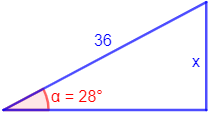
\includegraphics[scale=1]{P1.png}
\caption{Problema}
\end{figure}
\begin{figure}[H]
\centering
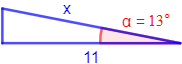
\includegraphics[scale=1]{P2.png}
\caption{Problema}
\end{figure}
\begin{figure}[H]
\centering
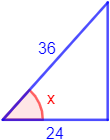
\includegraphics[scale=1]{P3.png}
\caption{Problema}
\end{figure}
\begin{figure}[H]
\centering
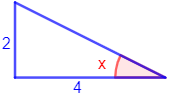
\includegraphics[scale=1]{P4.png}
\caption{Problema}
\end{figure}
\begin{figure}[H]
\centering
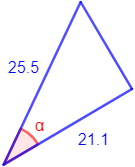
\includegraphics[scale=1]{P5.png}
\caption{Problema}
\end{figure}
\begin{figure}[H]
\centering
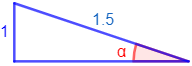
\includegraphics[scale=1]{P6.png}
\caption{Problema}
\end{figure}
\begin{figure}[H]
\centering
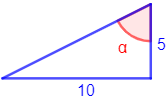
\includegraphics[scale=1]{P7.png}
\caption{Problema}
\end{figure}
Las respuestas de las tareas pueden ser enviadas al siguiente correo giovannilopez9808@gmail.com con el asunto entre corchetes de la siguiente manera [Tarea \#] y el nombre del archivo con sus apellidos y nombre, ya sea el nombre completo o solo una parte, por ejemplo \textit{LopezPadilla.pdf}, \textit{LopezGiovanni.pdf}, \textit{LopezPadillaGiovanniGamaliel.pdf}. Las respuestas envienlas en formato pdf, estas pueden ser totalmente digitales (que escriban todo en la computadora) o que sean fotografías, pero por favor, envielo en solo un documento.
\end{document}